\chapter{Обзорно-аналитическая часть}
\section{Существующие системы позиционирования}
На сегодняшний день, наибольшее распространение получили\cite{ruwikilbs} два вида систем позиционирования: основанные на спутниковой навигации и основанные на принимаемых уровнях сигналов от базовых станций сотовых сетей.

\subsection{Спутниковая навигация}
\label{subsec:satnav}
Спутниковые системы позиционирования, такие как GPS и ГЛОНАСС, в качестве опорных точек используют орбитальную группировку спутников, специально запущенных для целей навигации. Орбитальные элементы для всех спутников известны, а потому вычислить местонахождение каждого из них в любой момент времени возможно с большой точностью. После того, как они вычислены, можно осуществлять непосредственно позиционирование.

\begin{figure}[h]
	\center{
		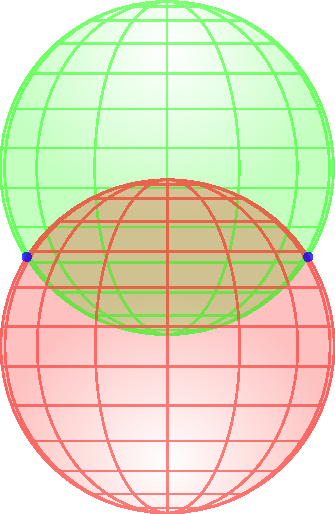
\includegraphics[width=0.4\linewidth]{Lat_2spheres_2.pdf}
		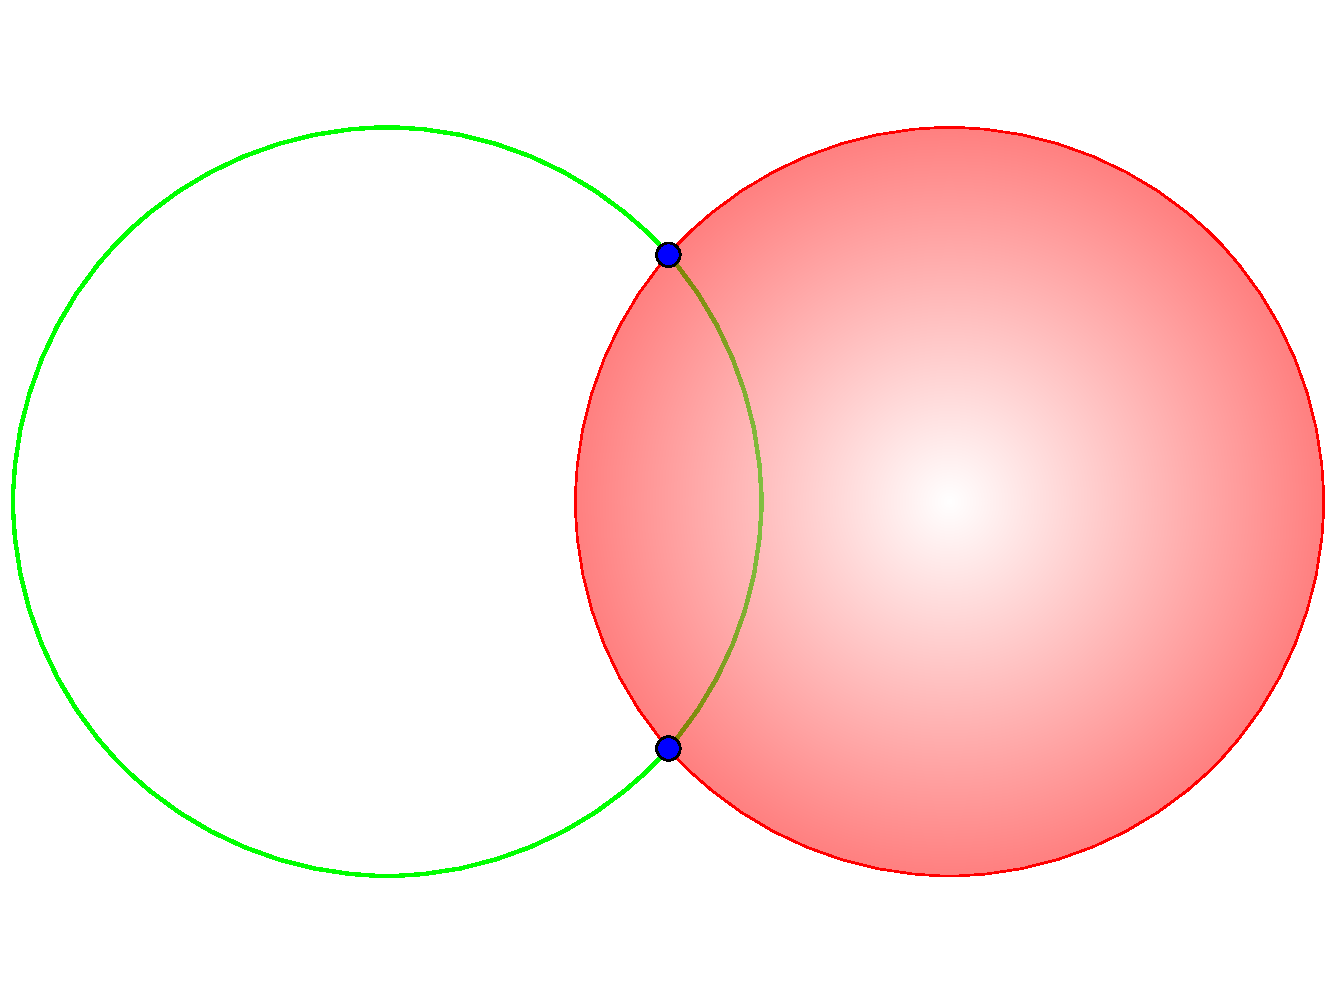
\includegraphics[width=0.4\linewidth]{Circle_sphere_2-colour.pdf}
	}
	\caption{Две пересекающиеся сферы образуют окружность. Третья сфера, пересекая эту окружность, образует две точки. Изображения из фонда Wikimedia Commons.}
	\label{fig:2-3-spheres-intersect}
\end{figure}
GPS использует метод трилатерации, в котором измеряется расстояние от приёмника до трёх видимых спутников. Три сферы, пересекаясь, дают две возможные точки, причём расположенные на разной высоте (см. рис. \ref{fig:2-3-spheres-intersect}), а потому правильной считается ближайшая к поверхности Земли. Для измерения расстояния оценивается время прохождения сигнала от спутника до приёмника. Средняя высота орбит спутников GPS над поверхностью Земли составляет порядка $2\cdot10^7$ метров\cite{enwikigps}, что, с учётом скорости света, равной $3\cdot10^8$ м/с, даёт характерное время прохождения сигнала около 60 миллисекунд. Чтобы при таком порядке задержки обеспечить достаточную точность позиционирования, все спутники оборудованы синхронизированными атомными часами, дающими точность около 14 наносекунд\cite{enwikigps}, причём для её обеспечения приходится учитывать эффекты специальной теории относительности, применительно к движению спутника. Было бы крайне дорого обеспечивать каждый приёмник такими же часами, а потому точное время он вычисляет каждый раз, когда принимает сигнал от спутника, решая уравнения метода трилатерации и относительно положения, и относительно времени.

В случае, когда в области видимости находится более, чем 4 спутника, система уравнений, описывающих положение приёмника, становится избыточной, количество уравнений превышает количества неизвестных. В этом случае, с одной стороны, можно выбрать набор спутников, использование которых даёт наибольшую точность позиционирования, оценивая величину геометрического ухудшения точности (geometric dilution of precision --- GDOP), с другой --- решать избыточную систему уравнений одним из приближённых численных методов, таких как метод наименьших квадратов, чтобы получить лучшую оценку положения автоматически\cite{enwikigps}.

Характерное же расстояние от мобильного устройства до базовой станции сотовой сети, в зависимости от стандарта, составляет $10^2$--$10^4$ метров. Для обеспечения соответствующей точности трилатерации в таких сетях, потребовалось бы пропорционально снизить погрешность точного времени, что представляется трудноосуществимым, поскольку для синхронизации часов базовых станций используется как раз сигнал GPS\cite{gsmclockcalibr}. В связи с этим, в отсутствие возможности использования сигнала GPS (отсутствие приёмника или видимости спутников), применяются иные методы.

\subsection{Позиционирование в сотовых сетях}
Как было показано в пункте \ref{subsec:satnav}, метод оценки расстояния между источником и приёмником, с помощью измерения задержки прохождения сигнала для сотовых сетей неприменим. Однако, остаётся возможность измерить амплитуду принимаемого сигнала, убывающую обратно пропорционально квадрату расстояния. Стандартный GSM-модуль может предоставить информацию об амплитуде принимаемого сигнала не только от базовой станции, через которую идёт передача данных, но и обо всех окружающих, сигнал которых можно принять. Информация эта представляется в виде логарифмической величины received signal strength indicator (RSSI), преобразованную из стандартной единицы измерения --- децибел мощности (dBm) --- в дискретную единицу измерения asu, представляющую из себя целое число в диапазоне от 0 до 31, где 0 соответствует самому малому уровню сигнала, доступному в шкале, а 31 --- самому большому\cite{androidnecelinf}.

\subsubsection{Распространение сигнала на открытой местности}
Максимальный радиус действия одной базовой станции в сети GSM составляет 35 километров на открытой местности, а в условиях городской застройки плотность их расстановки может составлять вплоть до одной станции на 400 метров\cite{enwikicellsite}. Максимальная излучаемая мощность базовой станции стандарта DCS 1800 составляет 40 Вт\cite{gsmts}. Длина волны частотой 1800 МГц составляет $3\cdot10^8\text{(м/с)}/1800\cdot10^6\text{(Гц)} = 16\text{(см)}$. Примем эту величину за характерный размер излучателя и вычислим плотность потока электромагнитного излучения, считая, что 40 Вт излучения проходят через сферу диаметром 16 см:
\begin{equation}
	\label{eq:40wdensity}
	\frac{40\text{(Вт)}}{\pi\cdot0,16^2\text{(м)}} = 497\text{(Вт/м}^2\text{)}
\end{equation}
Отсюда, зависимость мощности излучения от расстояния до базовой станции составит:
\begin{equation}
	\label{eq:p40ofr}
	P = \frac{40^2}{497\cdot{}\pi{}\cdot{}R^2}
\end{equation}
Построим график этой зависимости.

\begin{figure}[h]
	\center{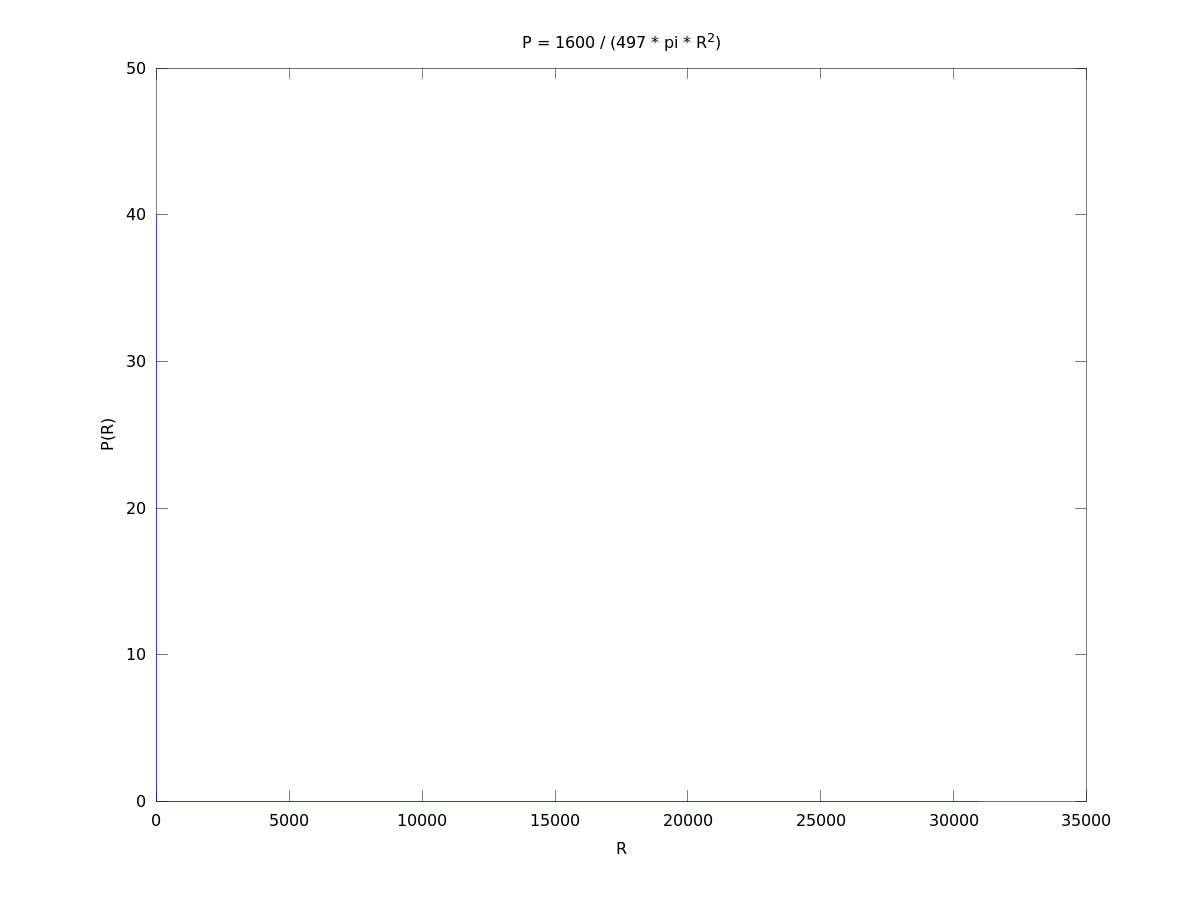
\includegraphics[width=1\linewidth]{bs40wp.png}}
	\caption{Зависимость мощности излучения в ваттах от расстояния в метрах до базовой станции GSM DCS 1800 мощностью 40 Вт. Гипербола столь быстро сходится к асимптотам, что на рисунке сливается с осями координат.}
	\label{fig:bs40wp}
\end{figure}

На рис. \ref{fig:bs40wp} видно, что мощность, измеренная в ваттах, близка к нулю для всех 35 возможных километров. В связи с этим, целесообразно введение логарифмической величины децибел мощности (dBm), связанной с ваттом следующим соотношением\cite{enwikidbm}:
\begin{equation}
	\label{eq:wtodbm}
	x = 10\cdot{}\log_{10}(1000\cdot{}P)
\end{equation}
Подставим формулу \ref{eq:p40ofr} в \ref{eq:wtodbm} и построим график получившейся зависимости.

\begin{figure}[h]
	\center{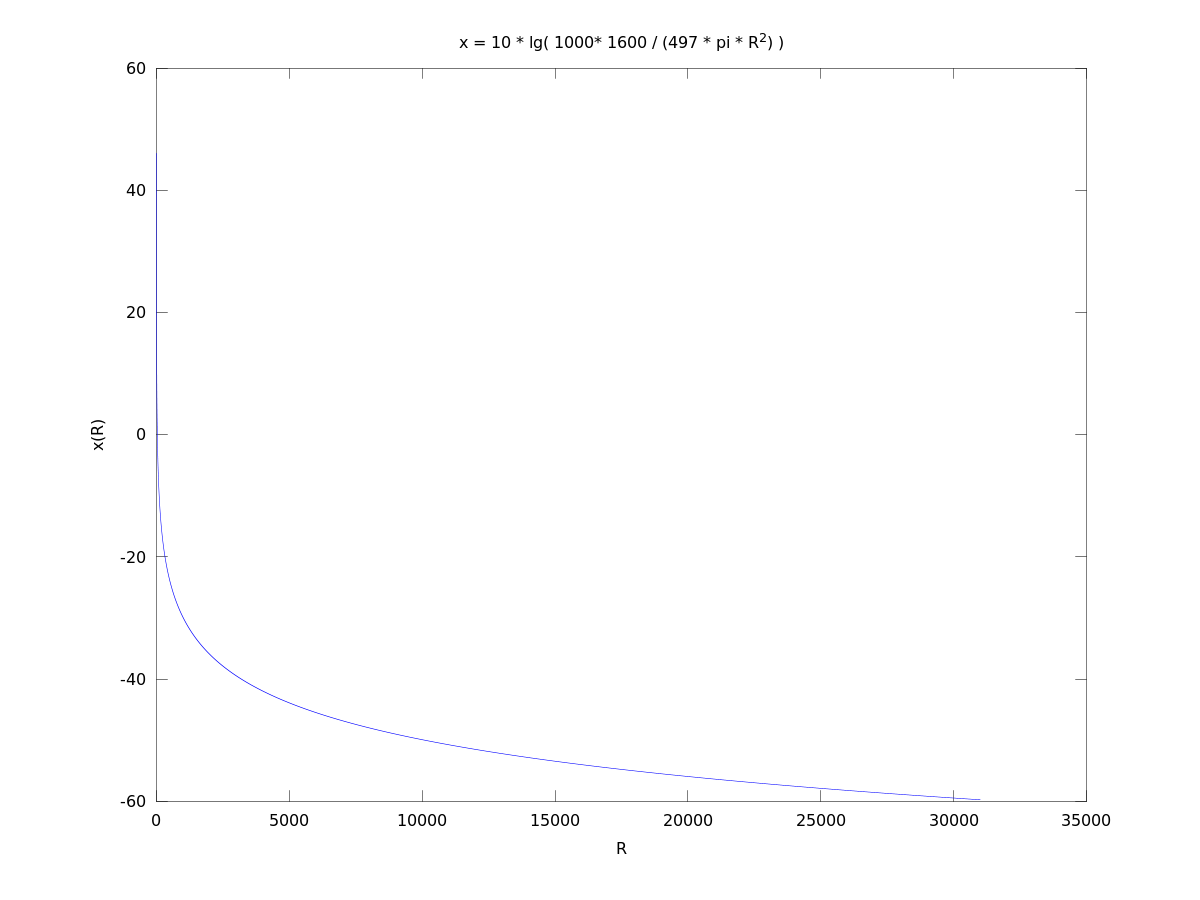
\includegraphics[width=1\linewidth]{bs40wdbm.png}}
	\caption{Зависимость мощности излучения в децибелах мощности от расстояния в метрах до базовой станции GSM DCS 1800 мощностью 40 Вт.}
	\label{fig:bs40wdbm}
\end{figure}

На рис. \ref{fig:bs40wdbm} видно, что использование логарифмического масштаба позволяет получить кривую, намного более равномерно заполняющую координатную плоскость, чем в линейном масштабе как на рис. \ref{fig:bs40wp}.

Наконец, возьмём связь между единицами dBm и asu\cite{androidnecelinf}:
\begin{equation}
	\label{eq:dbmtoasu}
	\text{asu} = \frac{\text{dBm} + 113}{2}
\end{equation}
Подставим формулы \ref{eq:p40ofr} и \ref{eq:wtodbm} в \ref{eq:dbmtoasu} и получим:
\begin{equation}
	\label{eq:p40rtoasu}
	\text{asu} = \frac{10\cdot{}\log_{10}(1000\cdot{}\frac{40^2}{497\cdot{}\pi{}\cdot{}R^2}) + 113}{2}
\end{equation}

\subsubsection{Погрешность определения расстояния}
Рассмотрим формулу \ref{eq:p40rtoasu} и найдём, на каких расстояниях от базовой станции будет меняться asu.
\begin{table}
	\caption{\label{tab:asuchange}Расстояния до точек изменения asu от базовой станции GSM DCS 1800 мощностью 40 Вт. Теоретическая оценка.}
	\begin{center}
		\begin{tabular}{|p{0.2\linewidth}|l|p{0.2\linewidth}|p{0.3\linewidth}|}
			\hline
			Расстояние от станции, метров & Значение asu & Расстояние до следующей точки изменения asu & Отношение расстояния до следующей точки изменения asu к расстоянию от станции \\
			\hline
			143 & 50 & 37 & 0.259 \\
			\hline
			180 & 49 & 47 & 0.261 \\
			\hline
			227 & 48 & 58 & 0.255 \\
			\hline
			285 & 47 & 74 & 0.260 \\
			\hline
			259 & 46 & 93 & 0.259 \\
			\hline
			359 & 46 & 93 & 0.259 \\
			\hline
			452 & 45 & 117 & 0.259 \\
			\hline
			569 & 44 & 148 & 0.260 \\
			\hline
			717 & 43 & 185 & 0.258 \\
			\hline
			902 & 42 & 234 & 0.259 \\
			\hline
			1136 & 41 & 294 & 0.259 \\
			\hline
			1430 & 40 & 370 & 0.259 \\
			\hline
			1800 & 39 & 466 & 0.259 \\
			\hline
			2266 & 38 & 587 & 0.259 \\
			\hline
			2853 & 37 & 739 & 0.259 \\
			\hline
			3592 & 36 & 930 & 0.259 \\
			\hline
			4522 & 35 & 1170 & 0.259 \\
			\hline
			5692 & 34 & 1475 & 0.259 \\
			\hline
			7167 & 33 & 1856 & 0.259 \\
			\hline
			9023 & 32 & 2336 & 0.259 \\
			\hline
			11359 & 31 & 2941 & 0.259 \\
			\hline
			14300 & 30 & 3700 & 0.259 \\
			\hline
			18000 & 29 & 4660 & 0.259 \\
			\hline
			22660 & 28 & 5870 & 0.259 \\
			\hline
			28530 & 29 & & \\
			\hline
		\end{tabular}
	\end{center}
\end{table}
В таблице \ref{tab:asuchange} для наглядности мы намеренно пренебрегли ограничением на максимальное значение asu, равное 31, и это допустимо, поскольку при использовании базовой станции с меньшей мощностью передатчика, значения asu также сдвинутся в меньшую сторону, и допустимый диапазон asu будет достигаться не на границе радиуса действия базовой станции, а в его середине или начале.

\begin{figure}[h]
	\center{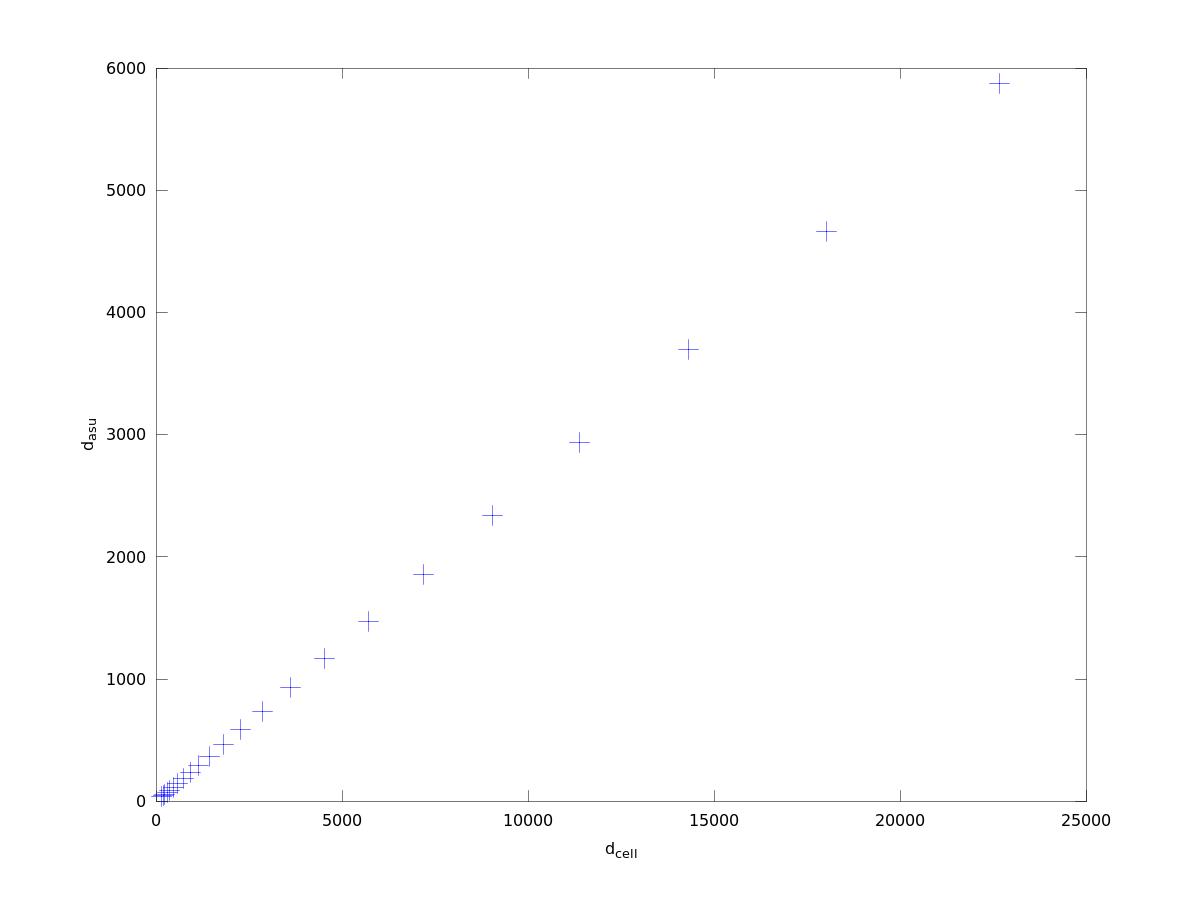
\includegraphics[width=1\linewidth]{dcelldasu.png}}
	\caption{Зависимость расстояния между двумя точками, где asu принимает целочисленное значение, от расстояния этих точек до базовой станции, по осям отложены метры}
	\label{fig:dcelldasu}
\end{figure}

Поскольку GSM-модуль передаёт для дальнейшей обработки только целую часть asu, расстояние между двумя соседними точками, где asu на самом деле имеет целое значение, можно считать погрешностью изменения расстояния на этом интервале. А так как измеряемой величиной является расстояние до базовой станции, отношение длины этого интервала к расстоянию до неё будет относительной погрешностью измерения. Из таблицы \ref{tab:asuchange} видно, что относительная погрешность остаётся постоянной на любом расстоянии. На рис. \ref{fig:dcelldasu} наглядно показано, что абсолютная погрешность при этом, как и следует ожидать, зависит от расстояния линейно.

При этом, стоит заметить, что эти значения погрешности были вычислены в предположении, что единственным фактором, ограничивающим точность измерений, является <<цена деления>> GSM-модуля, измеряющего asu. Однако в реальности, следует ожидать вмешательства случайной погрешности. Если считать, что в некоторой местности уровень электромагнитных помех примерно одинаков для любой точки, то с ростом расстояния до базовой станции отношение сигнал/шум будет падать, что внесёт дополнительную погрешность.

Таким образом, видно, что измерение расстояния от базовой станции до мобильного устройства, основанное на амплитуде сигнала, позволяет достигнуть точности от десятков метров до единиц километров, в зависимости от расстояния до базовой станции и мощности её передатчика. Наибольшая точность достигается вблизи станции, но при условии, что измеренное значение RSSI, выраженное в единицах asu, не выходит за пределы допустимого диапазона.

\subsubsection{Координаты базовых станций}
Для определения абсолютного местоположения мобильного устройства, а не только его положения относительно некоторых опорных точек, требуется знать координаты самих опорных точек. В случае использования спутниковой навигации, спутники немногочисленны --- на 24.05.2010 их было 31\cite{enwikigps} на всю Землю --- а их координаты в любой момент времени можно рассчитать с помощью законов орбитальной механики. В случае же базовых станций сотовых сетей, их количество для одной только России на конец 2011 года превысило 165 тысяч\cite{decodcells}. При этом, популярными провайдерами геолокационных сервисов зачастую являются не сотовые операторы, а сторонние компании, такие как Google, предоставляющий сервис Google Latitude, или Яндекс.Локатор от компании Яндекс\cite{ruwikilbs}. Такие провайдеры могут работать в зонах покрытия множества различных операторов сотовой связи, а также, при наличии соответствующего приёмного оборудования на мобильном устройстве, использовать для повышения точности позиционирования и другие беспроводные сети, такие как WiFi или WiMAX\cite{geolocationapidata}\cite{googlocsource}. 

В связи с этим, у провайдера геолокационного сервиса обычно нет априорных данных о координатах базовых станций, которые используются для позиционирования. Работа любой подобной системы начинается с того, что измеряются RSSI видимых базовых станций во множестве точек на местности, координаты которых получаются с помощью спутниковой навигации. Когда достаточное количество подобных замеров осуществлено, решается обратная задача -- вместо позиционирования устройства по известным координатам базовых станций, приближённо вычисляются координаты базовых станций, при известных координатах точек замеров RSSI.\cite{talberg}. Также распространена ситуация, в которой данные о координатах базовых станций уточняются непосредственно в процессе работы системы. В этом случае, провайдеры изыскивают способы вынудить самих пользователей сервиса посылать данные, помогающие уточнить базу данных. Так, пользовательское соглашение сервиса Яндекс.Локатор требует обязательной посылки данных нетмониторинга в случае, если от пользователя к сервису поступает более тысячи запросов в день\cite{yaloceula}.

Поскольку предполагаемые координаты базовых станций представляют собой большой объём данный, к тому же, постоянно изменяющийся, они хранятся не на позиционируемом устройстве, а на сервере провайдера геолокационного сервиса. Таким образом, само устройство вычислить свои координаты не может, оно лишь отправляет запрос с результатами измерений на сервер, откуда получает ответ о предполагаемом местонахождении\cite{yageloc}. Поэтому для работы таких систем обязательно наличие подключения к интернету.

Отсюда следует, что:

\begin{enumerate}
	\item
		Подобные системы являются самообучающимися: чем больше их используют, тем точнее они работают;
	\item
		Подобные системы могут работать только в тех местах, где кто-то ранее измерял RSSI и посылал эти данные провайдеру вместе с определёнными по GPS координатами точки измерения.
\end{enumerate}

\subsubsection{Факторы, снижающие точность позиционирования}
\label{subsubsec:pospreclow}
Реальные условия работы системы могут существенным образом отличаться от рассмотренного случая. В силу ряда факторов, системы позиционирования в мобильных сетях не достигают такой точности, как спутниковые. В отличие от спутниковых систем, сигналы точного времени которых могут быть либо приняты, либо нет, а на время прохождения сигнала влияет только расстояние, уровень сигнала от станций сотовых сетей подвержен множеству аналоговых искажений. Сюда можно включить:

\begin{enumerate}
	\item
		Поглощение излучения городской застройкой, деревьями, атмосферными осадками;
	\item
		Частичное отражение излучения от городской застройки, в результате которого сигнал от базовой станции достигает мобильного устройства не по прямой, а по ломанной, причём иногда, в результате частичного отражения, одновременно несколькими путями;
	\item
		Волновые эффекты распространения сигнала между домами и воздушными силовыми и сигнальными кабелями, которые могут работать как волноводы;
	\item
		Анизотропия диаграммы направленности базовых станций, в связи с которой на одном и том же расстоянии от неё, но в разных точках, RSSI может быть разным;
	\item
		Анизотропия диаграммы направленности мобильных устройств, в связи с которой одно и то же устройство в одном и том же месте может показывать различные RSSI для всех окружающих базовых станций, в зависимости от своей ориентации в пространстве;
	\item
		Помехи на частотах работы базовых станций.
\end{enumerate}

Эти и многие другие факторы могут приводить сразу к двум негативным последствиям:

\begin{enumerate}
	\item
		На этапе сбора данных, искажённые RSSI приведут к ошибочному определению координат базовых станций:
	\item
		На этапе позиционирования мобильных устройств, точность будут снижать и ошибки в определении текущих уровней сигналов, и ранее накопленные ошибки позиционирования базовых станций.
\end{enumerate}

\subsection{Заключение}
\begin{table}
	\caption{\label{tab:gpsvslbs}Сравнение свойств спутникового позиционирования и позиционирования в сотовых сетях}
	\begin{center}
		\begin{tabular}{|p{0.2\linewidth}|p{0.3\linewidth}|p{0.3\linewidth}|}
			\hline
			Характеристика & GPS & Сотовые сети \\
			\hline
			Опорные точки & Десятки спутников на околоземных орбитах & Сотни тысяч стационарных базовых станций \\
			\hline
			Метод определения расстояния & Измерение задержки прохождения сигнала & Измерение затухания амплитуды сигнала \\
			\hline
			Координаты опорных точек & Известны с большой точностью & Необходимо приблизительно оценивать с помощью дополнительных измерений \\
			\hline
			Погрешность позиционирования & Единицы--десятки метров, зависит от видимости спутников & Десятки--сотни метров, зависит от множества факторов \\
			\hline
			Покрытие & Всемирное & Только там, где проводились предварительные замеры сигнала \\
			\hline
			Автономность устройства & Для работы достаточно приёмника & Нужен обмен данными с сервером провайдера \\
			\hline
			Условие прохождения сигнала & Нахождение под открытым небом с таким углом обзора, чтобы были видны хотя бы три спутника & Везде, где есть сотовая связь \\
			\hline
		\end{tabular}
	\end{center}
\end{table}

В таблице \ref{tab:gpsvslbs} сведены характеристики, рассмотренные в данном разделе. Видно, что спутниковая навигация выигрывает у позиционирования в сотовых сетях практически по всем параметрам. К её недостаткам можно отнести необходимость нахождения под открытым небом для работы спутниковой навигации, а в случае использования в автономных устройствах --- наличие приёмника GPS помимо и так необходимого модуля GSM, что повышает стоимость и энергопотребление прибора.

\section{Позиционирование общественного транспорта}

Позиционирование транспортных средств с помощью установленных на них автономных <<маяков>> является частным случаем задачи позиционирования мобильных устройств. В случае работы с легковыми и грузовыми автомобилями, требования не будут существенно отличаться от задачи позиционирования мобильного телефона или навигатора. Однако, если речь идёт об общественном транспорте, в задаче появляется новая сущность --- маршрут, от движения по которому транспортное средство не может отклоняться.

Трамвай не может отклониться от маршрута вообще, троллейбус --- не более, чем на длину штангового токоприёмника, автобус --- на ширину проезжей части. Иными словами, задачу позиционирования общественного транспорта можно считать практически одномерной. Для каждого транспортного средства маршрут движения известен заранее, определять его не требуется. Таким образом, возможность позиционирования устройства в произвольном месте двухмерной карты является избыточной по отношению к данной задаче.

\subsection{Снижение точности из-за двухмерной избыточности}
\label{subsec:2dlowprec}
\begin{figure}[h]
	\center{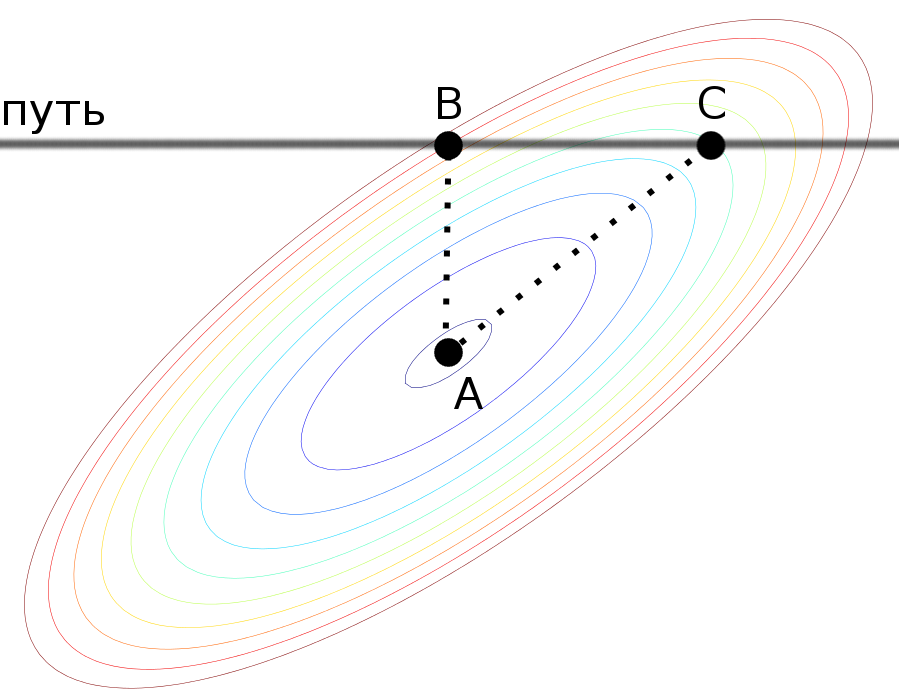
\includegraphics[width=1\linewidth]{contour.png}}
	\caption{Возможная ситуация при позиционировании транспорта. Изолинии показывают целевую функцию метода наименьших квадратов. Точка A --- глобальный минимум, она будет считаться результатом позиционирования. B --- проекция минимума на путь, по которому движется транспортное средство. C --- точка на пути движения, в которой достигается наименьшее значение целевой функции.}
	\label{fig:contour}
\end{figure}

Рассмотрим случай движения транспортного средства по прямой и позиционирования на ней. Как было отмечено в пункте \ref{subsec:satnav}, в случае, когда имеются избыточные данные о расстояниях до опорных точек, применяются различные методы приближённого решения, такие как метод наименьших квадратов. Конечным этапом применения такого метода будет определение для каждой точки на карте целевой функции, выражающей степень неуверенности в том, что данная точка является искомой, и поиск глобального минимума этой функции\cite{enwikiols}. На рис. \ref{fig:contour} изображено одно из возможных взаимных расположений пути следования транспортного средства и целевой функции. Глобальный минимум, который геолокационный сервер выдаст в качестве ответа на запрос местоположения, из-за ошибок измерения, находится в точке A, не лежащей на маршруте, хотя на самом деле, истинное положение находится где-то на маршруте. Если нам дана только точка A и маршрут движения, то наилучшим приближением будет проекция точки A на маршрут --- точка B. Однако, если учесть маршрут движения ещё на этапе, когда доступными являются все значения целевой функции, а не только информация о расположении минимума, то можно вычислить точку C, рассмотрев все точки, лежащие на маршруте, и найдя среди них такую, для которой значение целевой функции минимально, и это будет лучшим приближением.

\subsection{Снижение точности из-за экстраполяции}
\label{subsec:extralowprec}
Как было отмечено в подпункте \ref{subsubsec:pospreclow}, ошибки в ходе позиционирования возникают сразу на двух этапах: и на этапе составления карты базовых станций, и на этапе непосредственно позиционирования. Сам метод триангуляции обязывает применять именно такую последовательность действий, однако необходимо обосновать применение триангуляции как таковой. В случае позиционирования ручных и автомобильных устройств, необходимость применения этого метода обусловлена тем, что невозможно измерить уровни принимаемых сигналов во всех точках, где необходимо покрытие геолокационного сервиса. Так, если считать, что для триангуляции достаточно трёх замеров в точках, не лежащих на одной прямой, то для вычисления координат трёх базовых станций, достаточно трёх измерений, если учесть, что их зоны покрытия перекрываются. Три таких замера дадут возможность после этого позиционировать устройства во всей области, где перекрываются зоны покрытия этих станций.

В случае же общественного транспорта ситуация совершенно иная. Для примера рассмотрим московскую трамвайную сеть. На 46 маршрутов приходится 1000 трамваев\cite{ruwikimostram}. Если каждый трамвай хотя бы раз в день полностью проходит свой маршрут, это уже даст $1000/46 = 22$ вагона на одной линии. Приборы, оборудованные системой спутниковой навигации, и собирающие данные об RSSI, будучи установленными всего на один из каждых 22 вагонов, уже дадут полное обновление карты покрытия для каждой точки каждого маршрута.

Необходимости экстраполировать собранные данные на окружающие точки во всём городе в такой ситуации нет. Достаточно осуществить интерполяцию между имеющимися точками в одномерном случае.

\subsection{Гипотеза о возможности повышения точности}
Анализ факторов, изложенных в пунктах \ref{subsec:2dlowprec} и \ref{subsec:extralowprec}, позволяет предположить, что использование свойств, специфичных для наземного общественного транспорта, позволит отказаться от стадий процесса позиционирования, снижающих его точность. В данной работе экспериментально проверяется возможность этого.

\section{Анализ возможности применения существующих алгоритмов}
Рассмотрим, с помощью каких алгоритмов и математических методов можно решать задачу позиционирования, если не использовать триангуляцию.

\subsection{Постановка задачи}
\begin{enumerate}
	\item
		Дана числовая прямая, обозначающая маршрут движения. Задача отображения двухмерных координат на эту прямую решается отдельно;
	\item
		Некоторое количество переменных, выражающих принимаемый уровень сигнала от каждой станции, являются функциями от положения на прямой, определены на всей её длине (отсутствие сигнала можно трактовать как нулевой уровень), но подвержены также случайным флуктуациям;
	\item
		Для ряда точек, случайно расположенных на прямой, даны предварительно измеренные значения переменных. Возможна и ситуация неоднократных замеров в одной точке, давших разные результаты, они все попадают в массив измерений;
	\item
		Для кортежа из нескольких измеренных значений найти точку на прямой, где они с наибольшей вероятностью были осуществлены.
\end{enumerate}

Таким образом, требуется найти алгоритм, который будет способен сравнивать точки на прямой по степени их похожести друг на друга, основываясь на значениях набор дискретных, но упорядоченных переменных (то есть, учитывать то, что, например, 13 больше похоже на 14, чем на 42), устойчивый к выбросам (то есть, если какая-то одна станция неожиданно даст сигнал, резко отличающийся от своего нормального значения, это не должно стать помехой) и учитывающий ситуацию в соседних точках (если в некоторой точке никогда не было зафиксировано некое конкретное значение RSSI, но метром больше и метром ближе --- было, то для данной точки оно также должно быть репрезентативным). Также желательно учесть распределение результатов измерений для каждой точки, хотя подойдёт и использование среднего значения.

Математического метода, удовлетворяющего всем перечисленным требованиям, найдено не было, однако рассмотрим ряд существующих, наиболее приближающихся к заданным требованиям, на основе которых в дальнейшем будет синтезироваться новый.

\subsection{Расстояние Махаланобиса}
\label{subsec:mahalanobis}
Расстояние Махаланобиса --- это обобщение Евклидовой метрики на случай, когда известно, что сравниваемые векторы состоят из случайных переменных\cite{mahalanobis}. Для одного из сравниваемых векторов определяется матрица ковариации его компонентов, таким образом чётко выражена разница между целым набором статистических данных об измерениях, сделанных в конкретной точке, и вектором, однократно измеренным во время позиционирования. В дальнейшем, эта матрица используется для того, чтобы определить величину дисперсии значений в направлении между сравниваемыми векторами. В случае, когда дисперсия мала (то есть, известно, что получение значений, сильно отличающихся от среднего, маловероятно), расстояние получается больше Евклидова, когда велика -- меньше. Определяется расстояние по формуле \ref{eq:mahalanobis}.

\begin{equation}
	D_M(x) = \sqrt{(x - \mu{})^\intercal{}\cdot{}S^{-1}(x-\mu)}
	\label{eq:mahalanobis}
\end{equation}
В формуле \ref{eq:mahalanobis}:
\begin{itemize}
	\item
		{\bf$D_M(x)$} --- расстояние Махаланобиса от вектора $x$ до вектора $\mu$;
	\item
		{\bf$x$} --- однократно измеренный вектор;
	\item
		{\bf$\mu$} --- вектор с известным распределением;
	\item
		{\bf$S$} --- матрица ковариации вектора $\mu$.
\end{itemize}

В поставленной задаче расстояние Махаланобиса можно вычислить для всех точек на маршруте, после чего найти среди них наименьшее --- оно и будет точкой наиболее вероятного местонахождения устройства. Оценивая его применимость, отметим, что такой метод идеально справляется с учётом статистических данных об измеренных уровнях, учитывает упорядоченность множества возможных значений уровней, средне справляется в выбросами: если для какой-то конкретной станции известно, что её сигнал в данной точке нестабилен, она будет учитываться с меньшим весом в конечном результате. Однако если выброс даст <<надёжная станция>>, он в значительной мере изменит оценку.

Главным недостатком является тот факт, что такой метод не позволяет учесть непрерывность самого маршрута. Расстояние Махаланобиса можно определить только для одной точки, не учитывая соседние, либо для интервала, в рамках которого точки будут неразличимыми. Если же в некоторой точке уровни не были измерены никогда, то она никогда не будет результатом позиционирования, даже если есть данные о двух соседних.

\subsection{Байесовский классификатор}
\label{subsec:bayes}
Задача позиционирования по своей сути схожа с задачей классификации: если рассматривать каждую точку на маршруте как класс, то он будет определён имеющимися статическими данными о замерах RSSI в данном месте, а само позиционирование будет отнесением вектора измеренных значений к одному из классов. По этой причине в обзор также включён Байесовский классификатор.

Байесовский классификатор обладает следующими свойствами\cite{akinator}:
\begin{itemize}
	\item
		Строится на основании ранее полученных экземпляров класса, даже если сами экземпляры сильно искажены флуктуациями; сложение большого их количества обеспечивает выявление скрытых закономерностей, характерных для класса;
	\item
		Крайне устойчив к выбросам; мерой веса каждой из переменных является то, в какой мере она уменьшает энтропию распределения вероятности отнесения примера к различным классам, поэтому чем в большей мере нормальные значения переменных свидетельствуют в пользу конкретного класса, тем меньший вес имеют выбросы;
	\item
		Позволяет учесть распределение переменных в экземплярах одного класса.
\end{itemize}

Критическим же недостатком этого классификатора является то, что он рассчитан на дискретные классы и дискретные значения переменных, не позволяя учесть не только соседние точки, но и ближайшие значения RSSI, упорядоченность множества значений переменных тут не учитывается.

С другой стороны, именно как попытка в некотором смысле обобщения Байесовского классификатора на непрерывный случай и был изобретён метод, предлагаемый в данной работе, и Байесовское понимание вероятности как степени уверенности в суждении, а не частоты появления события, легло в его основу.

